\documentclass[12pt, a4paper]{article}
\usepackage[utf8]{inputenc}
\usepackage{ragged2e}

\usepackage{graphicx, geometry, hyperref, wrapfig}
\usepackage[dvipsnames]{xcolor}

\definecolor{silver}{RGB}{200,200,200}
\hypersetup{colorlinks=true, linkcolor=RoyalBlue, urlcolor=RoyalBlue}

 \geometry{
 a4paper,
 total={175mm,257mm},
 left=20mm,
 top=15mm,
 }

\usepackage{xcolor} % for defining colour
\usepackage{titlesec} % for customizing sections

% \usepackage{times}        % Use Times New Roman font
% \usepackage{helvet}       % Use Helvetica font
\usepackage{palatino}

\usepackage[T1]{fontenc}

\setlength\parindent{0pt}

% %%%%%%%%%%%%%%%%%%%%%%%%%%%%%%%%%%%%%%%%%%%%%%%%%%%%%%%%%%%%%%
\titleformat{\section}
{\color{UM_DarkBlue}\normalfont\large\bfseries}
{\color{UM_DarkBlue}\thesection}{1em}{}

%%%%%%%%%%%%%%%%%%%%%%%%%%%%%%%%%%%%%%%%%%%%%%%%%%%%%%%%%%%%%%%
\definecolor{UM_Brown}{HTML}{3D190D}
\definecolor{UM_DarkBlue}{HTML}{2264B0}
\definecolor{UM_LightBlue}{HTML}{1CA9E1}
\definecolor{UM_Orange}{HTML}{fEB415}

%%%%%%%%%%%%%%%%%%%%%%%%%%%%%%%%%%%%%%%%%%%%%%%%%%%%%%%%%%%%%%%%

\newcommand{\eg}{{\it e.g.}}
\newcommand{\ie}{{\it i.e.}}

% %%%%%%%%%%%%%%%%%%%%%%%%%%%%%%%%%%%%%%%%%%%%%%%%%%%%%%%%%%%%%%
% \hypersetup{
%     draft=false,
%     final=true,
%     colorlinks=true,
%     citecolor=UM_DarkBlue,
%     anchorcolor=yellow,
%     linkcolor=UM_DarkBlue,
%     urlcolor=UM_DarkBlue,
%     filecolor=green,      
%     pdfpagemode=FullScreen,
%     bookmarksopen=false
%     }
\usepackage{amsmath,amsfonts,amssymb,bm}

%%%%%%%%%%%%%%%%%%%%%%%%%%%%%%%%%%%%%%%%%%%%%%%%%%%%%%%%%%%%%
% Sets and Notations
\newcommand{\reals}{\mathbb{R}}
\newcommand{\integers}{\mathbb{Z}}

%%%%%%%%%%%%%%%%%%%%%%%%%%%%%%%%%%%%%%%%%%%%%%%%%%%%%%%%%%%%%
% Vectors and Matrices
% \renewcommand{\vec}[1]{\bm{\mathrm{#1}}}
\newcommand{\dotp}{\,\boldsymbol{\cdot}\,}
\newcommand{\grad}[1]{\vec{\nabla}#1}
\renewcommand{\div}[1]{\vec{\nabla}\!\dotp\!\vec{#1}}
\newcommand{\curl}[1]{\vec{\nabla}\!\times\!\vec{#1}}



%%%%%%%%%%%%%%%%%%%%%%%%%%%%%%%%%%%%%%%%%%%%%%%%%%%%%%%%%%%%%
% Derivatives
\newcommand{\dv}[2]{\frac{d#1}{d#2}}
\newcommand{\ndv}[3][2]{\frac{d^{\,#1}#2}{d#3^{\,#1}}}

\newcommand{\pdv}[2]{\frac{\partial#1}{\partial#2}}
\newcommand{\npdv}[3][2]{\frac{\partial^{\,#1}#2}{\partial#3^{#1}}}
 
\title{OWO-GAship}
\author{Anik Mandal}
\date{January 2025}
\pagenumbering{arabic}

%====================================================================================================
\begin{document}

\begin{minipage}[t][][c]{0.1\textwidth}
    \begin{flushleft}
        
\includegraphics[height=2.5cm]{tex-resources/Ashoka Logo.png}
    \end{flushleft}
\end{minipage}
\begin{minipage}[t][][c]{0.85\textwidth}
    \begin{center}
        {\LARGE Oscillations, Wave and Optics}\\ \vspace{0.5em}
        \textsc{(Spring 2025)}\\
        \vspace{1em}
        \textbf{\Large ASSIGNMENT-0} \\
    \end{center}
\end{minipage}
\vspace{10pt}\\
\rule[0em]{\textwidth}{0.75pt}

\flushleft{Topics: Basic Math (Calculus, Taylor Series, Fourier Series, ODE)}\hfill 
Total Marks: 50   \\
\flushleft{Date: 23nd Jan, 2025}\hfill
\fbox{\textbf{\large 
Due: 23rd Feb, 2025} (EoD)}\\
\vspace{.2cm}
\rule[0em]{\textwidth}{1.75pt}
\vspace{-1cm}
%====================================================================================================
%====================================================================================================
\justifying

\section*{Problem-1 \hfill \textbf{[10]}}
\textbf{(a)} Solve $4y'' + 4y' + 37y=0$ and find y(x) for the given boundary conditions: \\
(i) $y(x=0)=0$,(ii) $y(x=\frac{\pi}{6})=exp(-\frac{\pi^2}{12})$.\\
Crosscheck the solution; check whether your solution satisfies the ODE.\hfill \textbf{3+2}\\

\noindent
\textbf{(b)} Make a hand-drawn plot of the solution in the x-y plane using the reference informations:\\
(i) $exp(-\frac{1}{2})\approx 0.6$, (ii) $exp(-\frac{5}{4})\approx 0.3$, (iii) $exp(-\frac{9}{4})\approx 0.1$\\
Also briefly mention how you are using the provided informations for plotting. \hfill\textbf{2+1}\\

\noindent
\textbf{(c)} Taylor expand the solution about x=0. (\textit{Error/deviation of the order $x^5$is acceptable}).\\
Also, estimate the leading order error term in your truncated Taylor series at x=1. \hfill \textbf{2}

%====================================================================================================
\section*{Problem-2 \hfill \textbf{[10]}}
\textbf{(a)} (i) $x=sint$, (ii) $y=cos2t$\\ 
plot these two equations in the t-x and t-y planes, respectively. (\textit{In range $t=[0, 2\pi]$}).\hfill \textbf{2+2}\\

\noindent
\textbf{(b)} For a constant t, you will get the x-value and y-value using those two equations.
Use a set of t-values to get a set of x-values and y-values. 
Use those x-values and y-values to find the trajectory of the particle in the x-y plane.\hfill\textbf{3}\\

\noindent
\textbf{(c)} You can also use the trigonometric identities to solve those two equations for t 
to get y as a function of x. Plot that function in the respective limits of x and y.
And check whether the plot is equivalent to the plot in section-(b).\hfill\textbf{3}

%====================================================================================================
\section*{Problem-3 \hfill \textbf{[10]}}

\textbf{(a)} Integrate the function $f(x) = x^2$ for the range of $x=[-\pi, \pi]$.\hfill\textbf{1}\\

\noindent
\textbf{(b)} considering $f(x)$ to be periodic, that means $f(x + 2\pi) = f(x)$.
\begin{figure}[h]
    \centering
    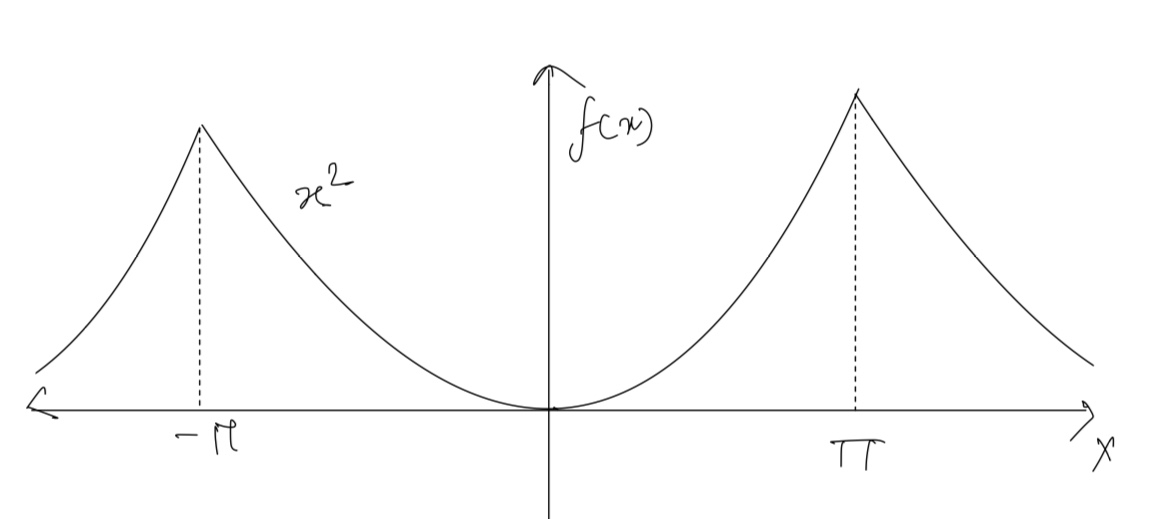
\includegraphics[scale=.25]{figs/a0-p3-x^2fourier.jpeg}
\end{figure}

\noindent
Find the Fourier series of the function. 
Determine whether it is necessary to evaluate the sine integral as part of the process,
and justify your answer with proper reasoning. \hfill\textbf{3+1}\\

\noindent
\textbf{(c)} Determine the number of terms n in the Fourier series expansion such that the leading-order
error is less than $0.1\%$ of the value of the truncated Taylor series at $x=\pi$.\hfill\textbf{3}\\

\noindent
\textbf{(d)} Integrate the truncated Fourier series in the same limit of x and determine the
deviation with respect to the integration result at part-(a). \hfill\textbf{2}\\
\textit{[You can use some advanced calculator or write a few lines of code to perform the term-wise summation. 
Just mention how you are doing the calculations.]}

%====================================================================================================
\section*{Problem-4: Calculate Integrals \hfill \textbf{[10]}}
\begin{enumerate}
    \item $\int (2cos2x - sin2x)\ e^{-x}\ dx$
    \item $\int sinx\ sin5x\ cos2x\ dx$
    \item $\int_{0}^{\infty}sinh3x\ e^{-2x}\ dx$
    \item $\int_{0}^{\pi}cos2x\ dx$
    \item $\int_{0}^{\pi}cos^{2}2x\ dx$
\end{enumerate}

%====================================================================================================
\section*{Problem-5: Solve the equations and find the roots \hfill \textbf{[6]}}
\begin{enumerate}
    \item $\int f(x)\ dx = cos4x + sin^{2}2x -1$ find $f(x)$.
    \item $\int f(x)\ dx = cos2x\ e^{-x} + t^5$ \textit{[t is independent of x]} find $f(x)$.
    \item $cos4x + sin^{2}2x-1 = 0$ find roots/ general solution.
\end{enumerate}
%====================================================================================================
\section*{Problem-6:  \hfill \textbf{[4]}}
Prove the relation:
\begin{equation*}
    cos\omega t  + cos(\omega t- \phi) + cos(\omega t- 2\phi) +...+ cos(\omega t- (n-1)\phi) = 
    \frac{sin(\frac{n\phi}{2})}{sin(\frac{\phi}{2})}cos(\omega t -\frac{1}{2}(n-1)\phi)
\end{equation*}\\
\textit{Hint: Try to use complex definition of $cos\theta$, rearrange the terms and use geometric series formula}.


\end{document}
